\documentclass[a4paper]{article}

\usepackage[utf8]{inputenc}
\usepackage[T1]{fontenc}
\usepackage{textcomp}
\usepackage[czech]{babel}
\usepackage{amsmath, amssymb}


% figure support
\usepackage{import}
\usepackage{xifthen}
\pdfminorversion=7
\usepackage{pdfpages}
\usepackage{transparent}
\newcommand{\incfig}[1]{%
    \def\svgwidth{\columnwidth}
    \import{./figures/}{#1.pdf_tex}
}

\pdfsuppresswarningpagegroup=1
\author{Hynek Kydlicek}
\title{Diskrétka 6}
\begin{document}
\maketitle
\section{Úkol 1}
Graf s takovým skóre určitě existuje viz obrázek \ref{fig:Souvisly graf}.
Avšak nesouvislý graf s takovým skóre existovat nemůže. Protože graf musí mít 8 vrcholů a největší stupeň grafu je 7,
musí existovat vrchol, který bude mít hranu s každým dalším vrcholem.
\begin{figure}[htpb]
    \centering
    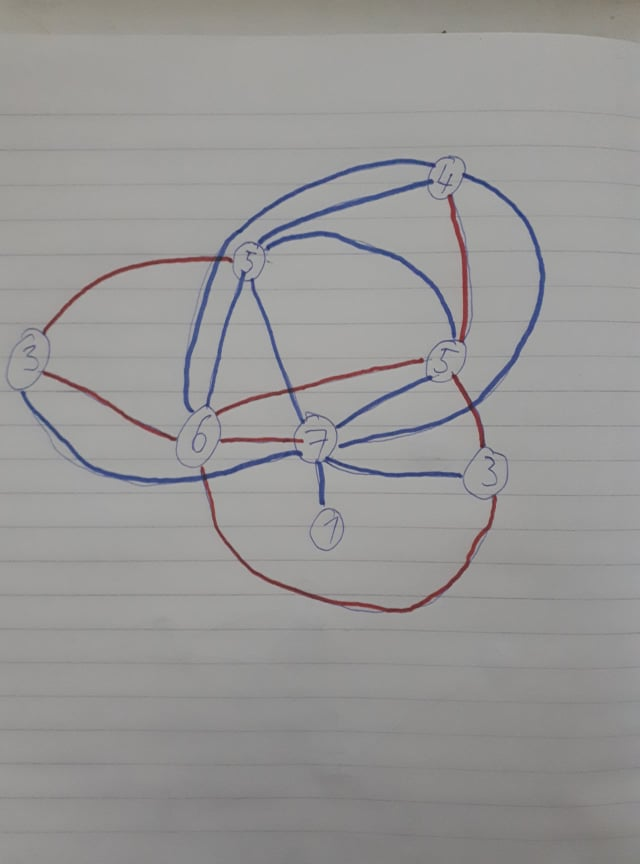
\includegraphics[width=0.5\textwidth]{ukol1.jpg}
    \caption{Souvislý graf}
    \label{fig:Souvisly graf}
\end{figure}
\section{Úkol 2}
Dokážeme sporem.
\\
Pro spor předpokládejme, že existuje souvislý graf $G(V,E)$ a existují dvě nejdelší cesty $P_1$, $P_2$ v $G$ a zároveň $P_1 \cap P_2 = \emptyset$.
\\
Pro $|V|$ = 1, dostáváme spor triviálně.
Předpokládejme proto $|V| \ge  2$
Jelikož je graf souvislý $\implies$ existuje cesta mezi každými 2 vrcholy grafu $G$. Z předpokladu $P_1 \cap P_2 = \emptyset$
dostáváme, že existují vrcholy $v_1 \in P_1, v_2 \in P_2$ a cesta $P_3$ s začátkem $v_1$ a koncem $v_2$
a $P_1 \cap P_3 = v_1 \wedge P_2 \cap P_3 = v_2$. Takovou cestu jsme schopni i zkonstruovat. Určitě existuje cesta $P$ mezi začátkem $P_1$ a koncem $P_2$. Pokud $|P_1 \cap P| > 1$ odeberem z $P$ začátek, tím snížíme mohutnost o 1 nebo 0.
Pokud $|P_2 \cap P| > 1$ odebereme z $P$ konec, tím snížíme mohutnost o 1 nebo 0. Protože $P_1 \cap P_2 = \emptyset$, odebráný vrchol $v$ má vlastnost $(v \in P_1 \wedge v \notin P_2) \vee (v \notin P_1 \wedge v \in P_2) \vee (v \notin P_1 \wedge v \notin  P_2)$.
Každý krok algoritmy sníží mohutnost jednoho z průniky o 0 nebo 1. Algoritmus končí pokud  $|P_1 \cap P| = 1 \wedge |P_2 \cap P| = 1$. Jelikož je cesta konečná algoritmus skončí vždy.
\\
\\
Označme si $a_1$ cestu $P_1$ od začátku do $v_1$, bez $v_1$.\\
Označme si $b_1$ cestu $P_1$ od konce do $v_1$, bez $v_1$.\\
Označme si $a_2$ cestu $P_2$ od začátku do $v_2$, bez $v_2$.\\
Označme si $b_2$ cestu $P_2$ od konce do $v_2$, bez $v_2$.\\
Označme si $d(P)$ délku cesty $P$, tedy počet vrcholů v $P$, tedy $|P|$.\\
Proto 
\begin{equation*}
    d(P_1) = d(a_1) + d(b_1) + 1 = d(P_2) = d(a_2) + d(b_2) + 1
\end{equation*}
BÚNO předpokladejme, že $d(a_1) \le d(a_2) \le  d(b_2) \le d(b_1)$
Vytvoříme novou cestu $P_g = b_1, P_3, b_2$. Z kontrukce víme, že každý vrchol se v cestě objeví maximálně jednou.
Zároveň víme, že $d(P_3) \ge  2$, protože musí obsahovat minimálně vrcholy $v_1,v_2$.
\begin{equation*}
    d(P_g) = d(b_1) + d(P_3) + d(b_2) \ge d(b_2) + d(P_3) + d(a_2) \ge d(b_2) + d(a_2) + 2 > d(P_2) = d(P_1)
\end{equation*}
Což je spor, předpokládali jsme, že $P_1,P_2$ jsou nejdelší cesty, ale našli jsme $P_3$, která je delší.
\end{document}
